\documentclass[aspectratio=169]{beamer}
\usepackage[utf8]{inputenc}
\usepackage{tikz}
\usepackage{tikz-cd}
\usepackage{tikz-layers}
\usepackage{pifont}
\usepackage{pgfpages}
\usepackage{pgfplots}
\usepackage{graphicx}
\usepackage[export]{adjustbox}
\usepackage{qrcode}
\usepackage{caption}
\usepackage{minted}
\usepackage[svgnames]{xcolor}
\usetikzlibrary{backgrounds}
\usetikzlibrary{decorations.pathreplacing}

% the drgtheme files live once at the repo root, in ../../../theme/
\makeatletter
\def\input@path{{../../../theme/}}
\makeatother
\graphicspath{{../images/}{../../../theme/}}

\usetheme{drgtheme}

%setup cover page variables
\title{MAC 233: Servo Lab}
\author{
    Dr Max Champneys
}
\institute[UoS]{
    School of Mechanical, Aerospace, and Civil Engineering,\\
    University of Sheffield, UK
}
\date{MAC 233: \hspace{0.1em}\textbf{28/10/2026}}
%setup footer variables
\runninginstitute{MAC 233, School of MAC, University of Sheffield}
\email{max.champneys@sheffield.ac.uk}

%Begin Document
\begin{document}

%Create Title Page
\maketitle

\begin{frame}{MAC 233: Labs Overview}
    \begin{center}
        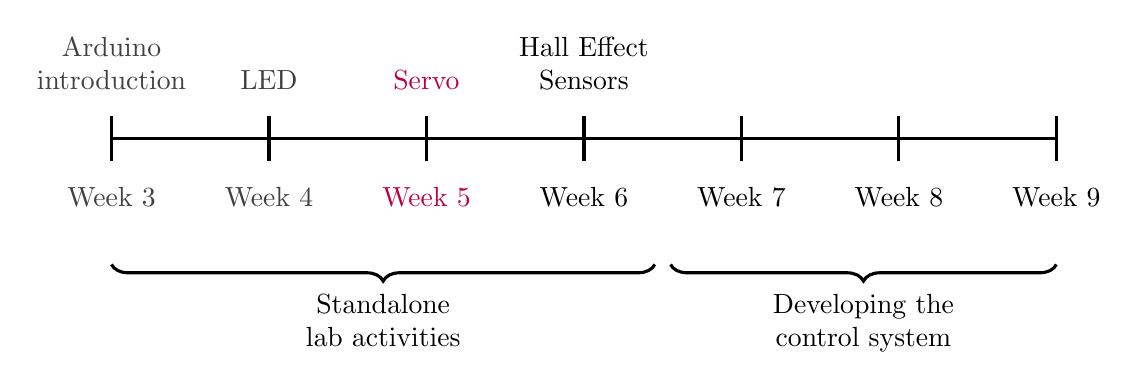
\begin{tikzpicture}[
            timeline/.style={color=black, line width=0.4mm},
            pastnode/.style={align=center, color=darkgray},
            currentnode/.style={align=center, color=purple},
            futurenode/.style={align=center, color=black}
        ]
            %line
            \draw[timeline] (-6, 0) -- (6, 0);

            % week ticks
            \foreach \x in {-6, -4, -2, 0, 2, 4, 6}{
                \draw[timeline] (\x, -0.28) -- (\x, 0.28);
            }

            % weeks (below the line)
            \node[pastnode, below] at (-6, -0.5) {Week 3};
            \node[pastnode, below] at (-4, -0.5) {Week 4};
            \node[currentnode, below] at (-2, -0.5) {Week 5};
            \node[futurenode, below] at (0, -0.5) {Week 6};
            \node[futurenode, below] at (2, -0.5) {Week 7};
            \node[futurenode, below] at (4, -0.5) {Week 8};
            \node[futurenode, below] at (6, -0.5) {Week 9};

            % activities (above the line)
            \node[pastnode, above] at (-6, 0.5) {Arduino\\introduction};
            \node[pastnode, above] at (-4, 0.5) {LED};
            \node[currentnode, above] at (-2, 0.5) {Servo};
            \node[futurenode, above] at (0, 0.5) {Hall Effect\\Sensors};

            % phases
            \draw[timeline, decorate, decoration={brace, amplitude=6pt, mirror}] (-6, -1.6) -- (0.9, -1.6);
            \node[futurenode, below] at (-2.55, -1.85) {Standalone\\lab activities};
            \draw[timeline, decorate, decoration={brace, amplitude=6pt, mirror}] (1.1, -1.6) -- (6, -1.6);
            \node[futurenode, below] at (3.55, -1.85) {Developing the \\ control system};

        \end{tikzpicture}
    \end{center}
\end{frame}

\begin{frame}{Today's Lab: Prerequisites}
    \Large
    This worksheet builds upon the theory of how to use an external pin that was covered in the Lab 2 worksheet. Whilst you won't need any code from Lab 2, you will need to have covered how to use a breadboard and how to wire up an external output to an Arduino pin. \\

    Out of your Arduino pack, you will need: 1 Arduino, 1 breadboard, 1 servo, and 3 jumper cables.
\end{frame}

\begin{frame}{Today's Lab: Objectives}
    \Large
    The objective of today's lab is to learn how to control a servo using the inbuilt Arduino Servo Library: \url{https://docs.arduino.cc/libraries/servo/}.\\

    The worksheet will take you through the steps of how to connect an external servo to your Arduino and create a sketch that rotates the servo in increments of 30 degrees.
\end{frame}

\begin{frame}{What is a servo?}
    \begin{center}
        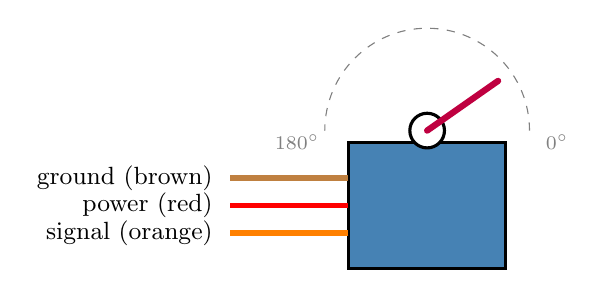
\begin{tikzpicture}[
            wire/.style={line width=.7mm},
            lbl/.style={font=\small, align=left},
        ]
            % sweep the arm can cover
            \draw[dashed, draw=gray] (2.1, 1.75) ++(0:1.3) arc (0:180:1.3);
            \node[font=\scriptsize, color=gray] at (3.75, 1.6) {$0^\circ$};
            \node[font=\scriptsize, color=gray] at (0.45, 1.6) {$180^\circ$};

            % body, output shaft and arm
            \filldraw[fill=SteelBlue, draw=black, line width=.4mm] (1.1, 0) rectangle (3.1, 1.6);
            \filldraw[fill=white, draw=black, line width=.4mm] (2.1, 1.75) circle (0.22);
            \draw[line width=.8mm, draw=purple, line cap=round] (2.1, 1.75) -- ++(35:1.1);

            % the three wires
            \draw[wire, draw=brown] (1.1, 1.15) -- (-0.4, 1.15);
            \draw[wire, draw=red]   (1.1, 0.8)  -- (-0.4, 0.8);
            \draw[wire, draw=orange](1.1, 0.45) -- (-0.4, 0.45);
            \node[lbl, anchor=east] at (-0.5, 1.15) {ground (brown)};
            \node[lbl, anchor=east] at (-0.5, 0.8)  {power (red)};
            \node[lbl, anchor=east] at (-0.5, 0.45) {signal (orange)};
        \end{tikzpicture}
    \end{center}

    \vspace{.5em}
    A servo is a motor with a gearbox and a small control circuit built into it. You tell it an \emph{angle}, and it turns to that angle and holds it there.

    \vspace{.5em}
    Two of its wires just supply power. The third carries the signal that tells the servo which angle you want.
\end{frame}

% [fragile] is required: the \verb commands below need it
\begin{frame}[fragile]{New: the Servo library}
    \large
    \begin{itemize}
        \setlength{\itemsep}{1em}
        \item \mintinline[fontsize=\large]{arduino}{#include <Servo.h>}\\
            makes the library available to your sketch
        \item \mintinline[fontsize=\large]{arduino}{Servo servo;}\\
            creates a servo for you to control
        \item \mintinline[fontsize=\large]{arduino}{servo.attach(SERVO_PIN);}\\
            says which pin the signal wire is on --- once, in \mintinline{arduino}{setup}
        \item \mintinline[fontsize=\large]{arduino}{servo.write(90);}\\
            moves the servo to an angle between 0 and 180 degrees
    \end{itemize}
\end{frame}

\begin{frame}[fragile]{What `servo.write' actually does}
    \begin{center}
        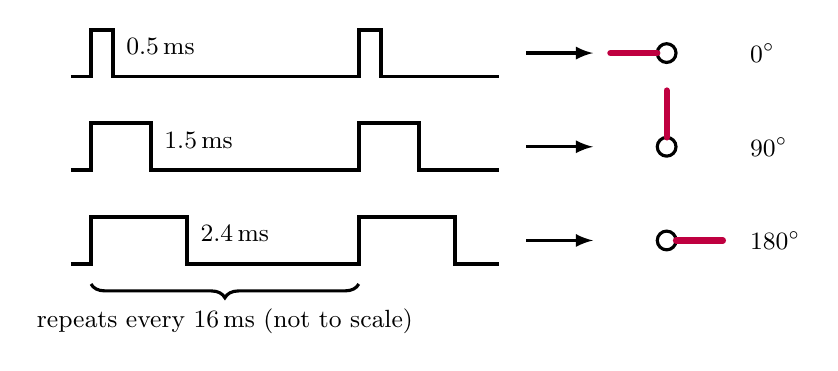
\begin{tikzpicture}[
            scale=.85,
            signal/.style={line width=.5mm, draw=black},
            arm/.style={line width=.8mm, draw=purple, line cap=round},
            lbl/.style={font=\small, align=center},
        ]
            % one row per angle: pulse width (1 ms = 0.6 units), row height, angle
            \foreach \w/\y/\ang/\ms in {0.33/0/0/0.5, 0.9/-1.4/90/1.5, 1.44/-2.8/180/2.4}{
                % two pulses of the repeating signal
                \draw[signal] (0, \y) -- (0.3, \y) -- (0.3, \y+0.7) -- (0.3+\w, \y+0.7) -- (0.3+\w, \y)
                    -- (4.3, \y) -- (4.3, \y+0.7) -- (4.3+\w, \y+0.7) -- (4.3+\w, \y) -- (6.4, \y);
                \node[lbl, right] at (0.35+\w, \y+0.45) {\ms\,ms};

                % the servo arm it produces
                \draw[-latex, line width=.4mm] (6.8, \y+0.35) -- (7.8, \y+0.35);
                \filldraw[fill=white, draw=black, line width=.4mm] (8.9, \y+0.35) circle (0.14);
                \draw[arm] (8.9, \y+0.35) ++(180-\ang:0.14) -- ++(180-\ang:0.7);
                \node[lbl, anchor=west] at (10, \y+0.35) {\ang$^\circ$};
            }

            % the repeat period
            \draw[line width=.4mm, decorate, decoration={brace, amplitude=5pt, mirror}] (0.3, -3.1) -- (4.3, -3.1);
            \node[lbl] at (2.3, -3.65) {repeats every 16\,ms (not to scale)};
        \end{tikzpicture}
    \end{center}

    \vspace{.25em}
    The Servo library sends a short 5\,V pulse every 16\,ms, and the \emph{width} of that pulse tells the servo which angle to turn to.
    % 20ms on some older AVR boards
    % note that this is MUCH slower than the 'true' servo

\end{frame}

\begin{frame}{Wiring Diagram}
    \vspace{-.5em}
    \begin{center}
        \begin{tikzpicture}[
            scale=1.65, transform shape, rotate=90,
            wire/.style={line width=.8mm},
            jumper/.style={draw=LimeGreen},
        ]

            %% mask out breadboard
            \filldraw[fill=white, draw=white] (0.54, -1.9) rectangle (1.04, -1.5);

            %% cables
            \draw[wire, jumper] (0.69, -1.75) -- (.607,-1.5) -- (.607, 0.604);
            \draw[wire, jumper] (0.792, -1.75) -- (.792, -0.49) to[out=130, in=50] (.42, -0.49) -- (-.87, -0.49) -- (-.87, 0.604);
            \draw[wire, jumper] (0.89, -1.75) -- (.975,-1.5) -- (.975, 2.08);

            %% components
            \draw[wire, draw=brown] (0.69,-2.32) -- (0.69, -1.75);
            \draw[wire, draw=red] (0.79,-2.32) -- (0.79, -1.75);
            \draw[wire, draw=orange] (0.89,-2.32) -- (0.89, -1.75);
            \filldraw[fill=black] (0.6, -1.8) rectangle (0.98, -1.6);
            \filldraw[fill=blue, draw=black] (-.15, -2.76) rectangle (1.05, -2.27);
            \filldraw[fill=white] (0.2,-2.51) circle (2mm);
            \node[] at (-.13, 1.43) {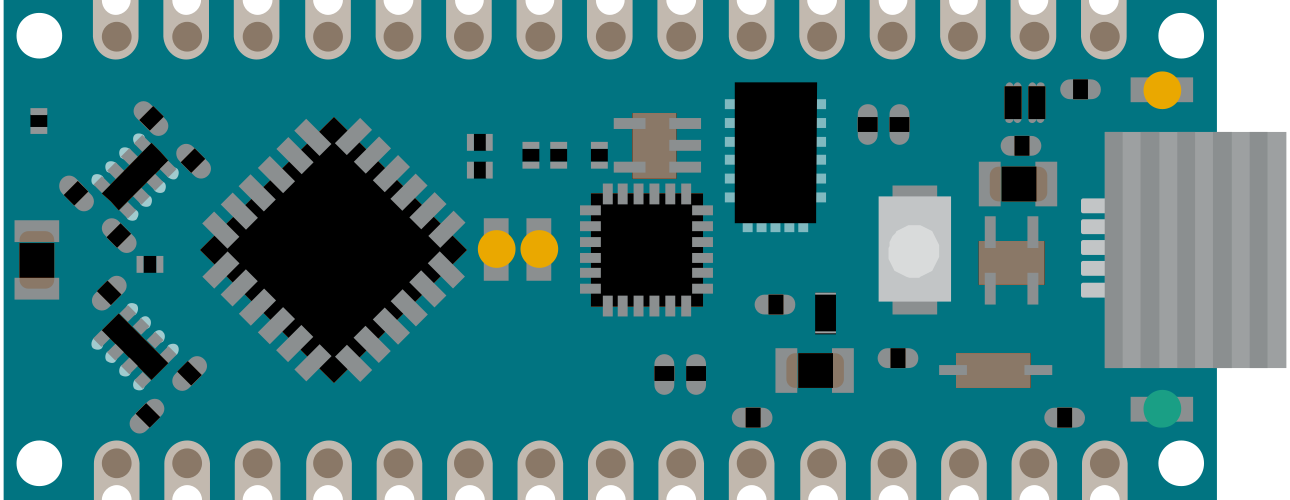
\includegraphics[angle=90, origin=c, width=3.38em]{../images/nano.png}};

            %% breadboard background
            \begin{scope}[on background layer]
                \node[] at (0, 0) {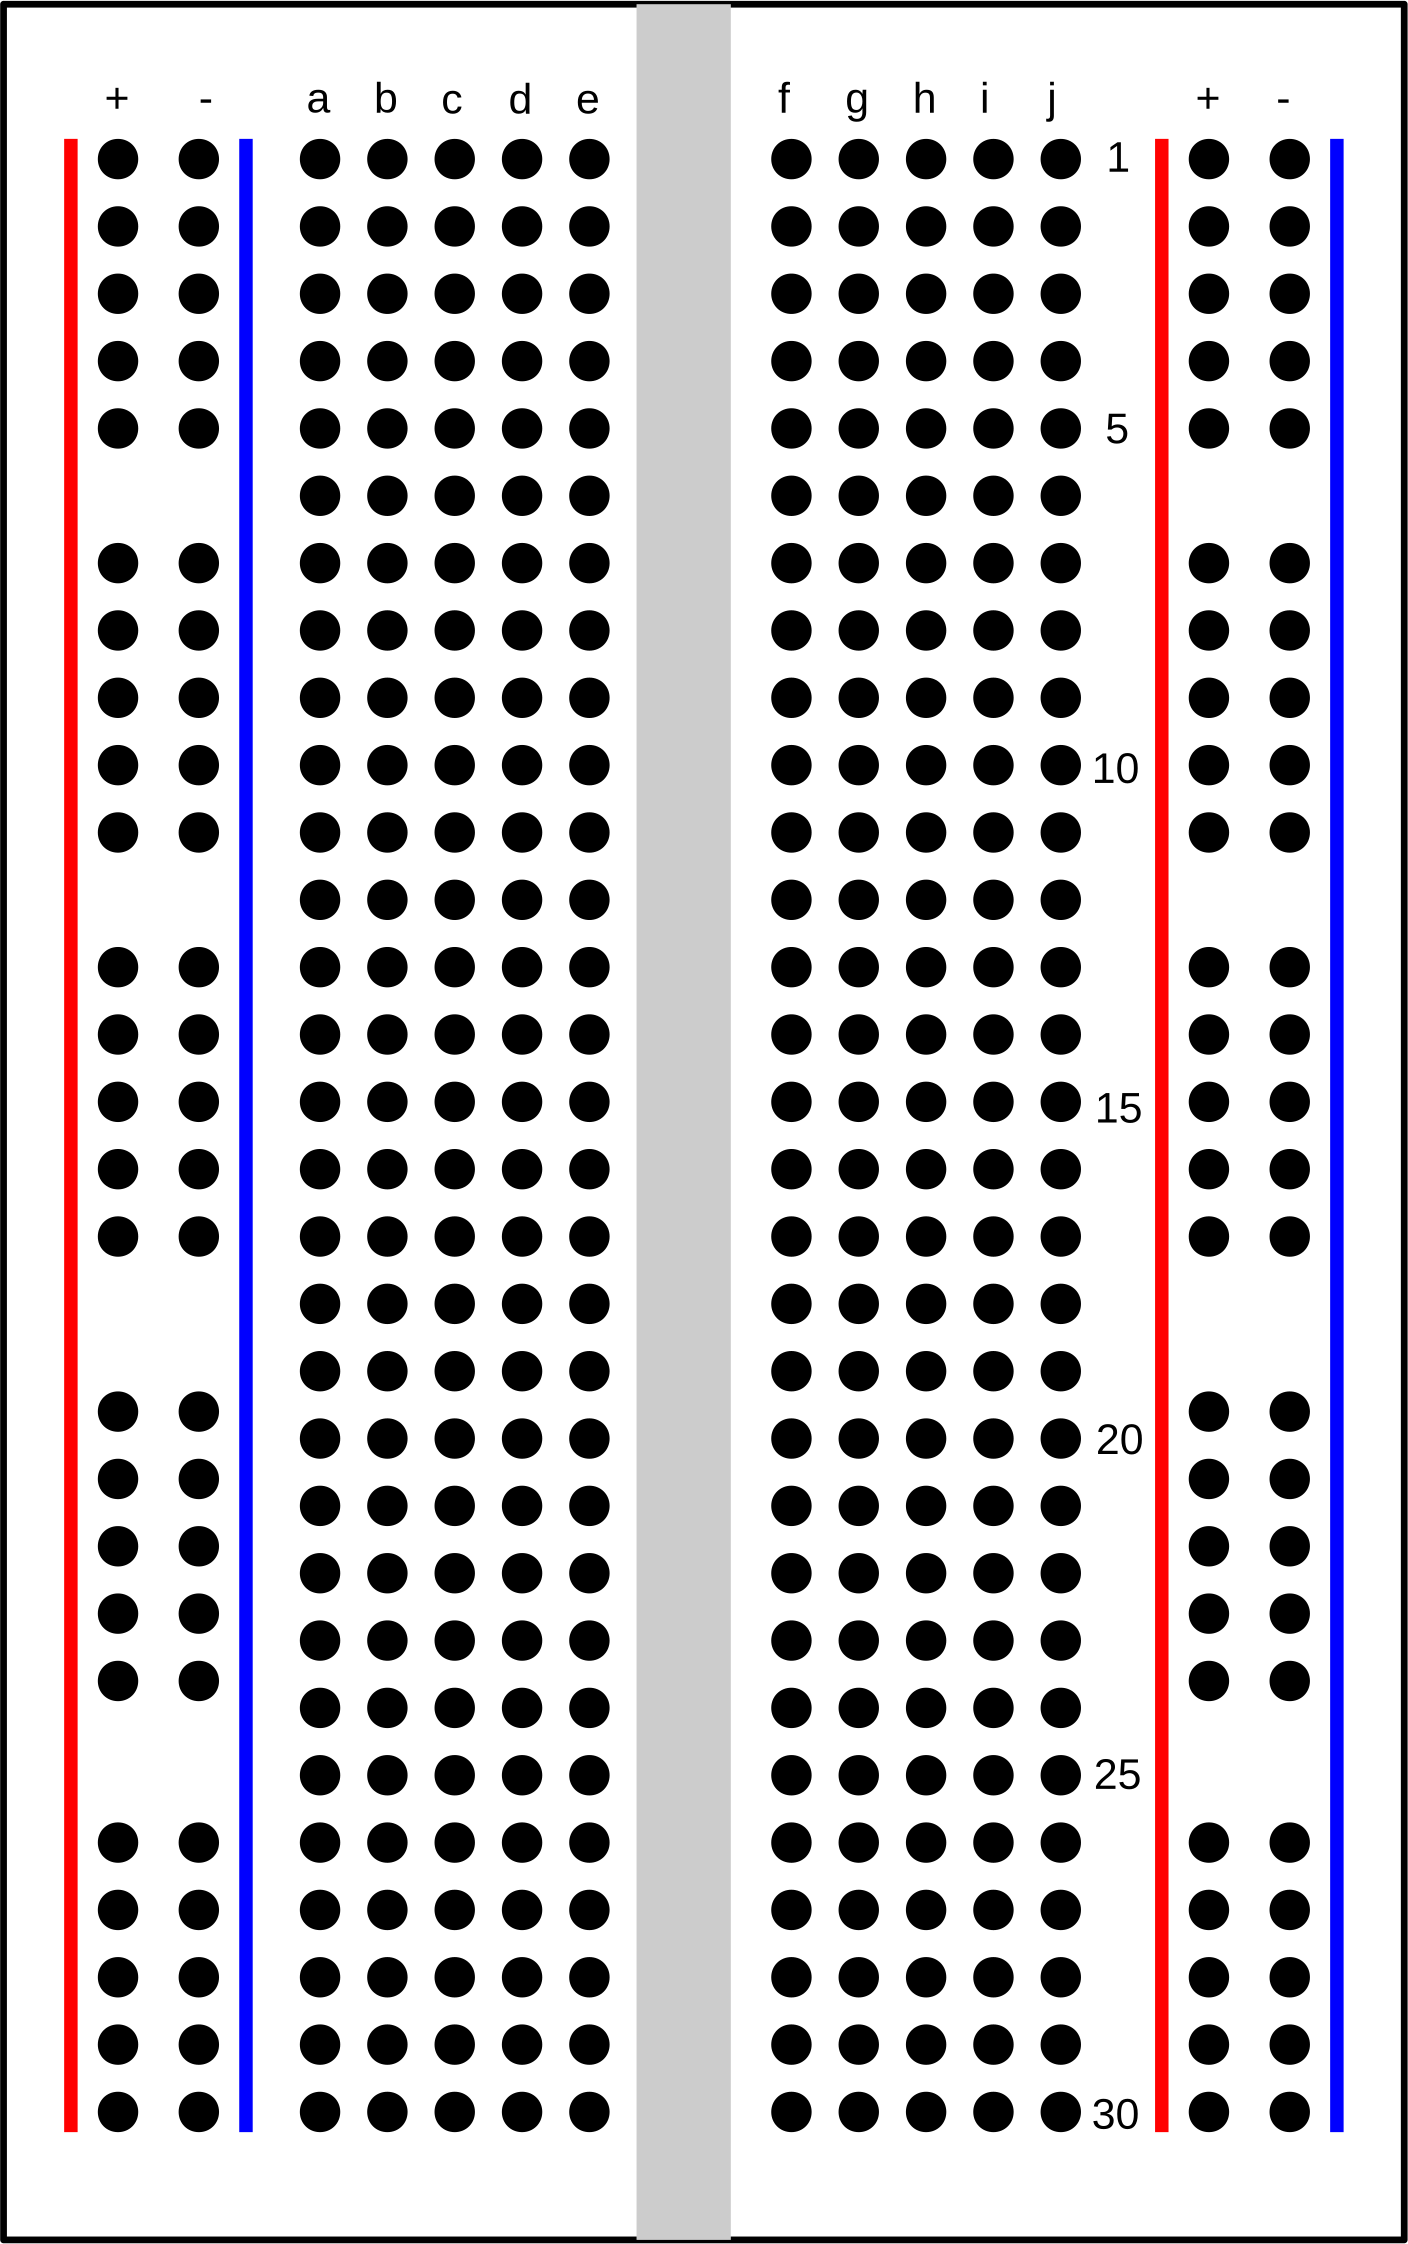
\includegraphics[width=10em]{../images/breadboard.png}};
            \end{scope}

        \end{tikzpicture}
    \end{center}
    \tiny
    Breadboard source: \url{https://freesvg.org/breadboard}.
\end{frame}

\begin{frame}{Help}
    \Large

    \normalsize
    \begin{columns}
        \begin{column}{.5\textwidth}
            \begin{center}
                \textbf{Lab 3 worksheet}\\
                \vspace{.5em}
                \qrcode[hyperlink, height=3cm]{https://github.com/MDCHAMP/MAC233/blob/main/labs/lab-3-servo/docs/lab-3-servo.pdf}
            \end{center}
        \end{column}
        \begin{column}{.5\textwidth}
            \begin{center}
                \textbf{Nano Every pinout}\\
                \vspace{.5em}
                \qrcode[hyperlink, height=3cm]{https://docs.arduino.cc/resources/pinouts/ABX00028-full-pinout.pdf}
            \end{center}
        \end{column}
    \end{columns}


    \vspace{3.5em}
    Problems? Raise your hand and someone will come and help you.

\end{frame}

\end{document}
